\chapter{基本概念}
\section{软件包及软件仓库}
\subsection{Ubuntu软件包}
Ubuntu软件包的文件格式不是常见的RPM格式,是DEB格式。DEB格式最早是由Debian使用,由于Ubuntu是从Debian分支发展而来,所以也继承了这种软件包格式。DEB软件包可以分为两类:扩展名为DEB的二进制软件包和扩展名为DSC的源码软件包。通常安装的软件只会用到二进制软件包,即DEB格式,而源码包只在查看、编译软件等特殊的时候才会用到。

\begin{itemize}
\item DEB软件包间的依赖关系

DEB软件包间常见的依赖关系有:Depends、Recommends和Conflicts。看这三个单词的字母意思就大致明白依赖关系是怎么回事了。假设有两个DEB软件包A和B:
\begin{itemize}
\item Depends:A依赖B,意味着安装软件包A时系统必须已安装软件包B;
\item Recommends:意味着开发这推荐用户在安装软件包A的同时也安装软件包B;
\item Conflicts:意味着软件包A和B不能共存,若软件包B已经安装,那么安装A的时候可能要自动卸载掉B。
\end{itemize}

\item DEB软件包的命名规则

对于常见的deb文件,命名规则如:\verb|gfce_ver-rev_arch.deb|

其中gfce是软件包的名字;ver代表版本;rev代表修订版本;arch是该软件包对应的硬件平台,如最常见的i386。
\end{itemize}


\subsection{软件仓库(软件源)}
软件仓库(软件源)是由Ubuntu软件包的维护者维护并公开发布的DEB软件包的集合,它可位于网络,如软件包服务器、HTTP、FTP服务器、光盘和硬盘等各种介质上。通常用户安装软件时不会自己下载DEB文件安装,而是由软件包管理工具根据用户的动作和配置计算依赖关系后,从软件仓库下载相应的软件包并安装。

显然软件仓库的一方面能保证大家用到安全的软件,降低了中病毒的风险;另一方面是方便大家安装使用软件,提高效率。软件仓库和苹果的软件商店等其他系统商店,本质是一样的,但后者是商业的。

需要注意的是:Ubuntu 和Debian都使用DEB软件包格式,但其软件仓库并不通用,不能把Debian的源设置为Ubuntu的源。


\section{Ubuntu实用工具}
\subsection{apt——高级软件包管理工具}
apt(Advanced Package Tool)工具可以完成所有的软件包的管理工作,包括维护系统中的软件包数据库、自动检查软件包依赖关系、安装和升级软件包、从软件源镜像站点主动获取相关软件包等。apt确切地说是一组命令的组合,这些命令组合又有若干参数,这样来完成各种工作。
\begin{itemize}
\item 安装
	\begin{itemize}
		\item \verb|apt-get install gfceu|,安装名为gfceu的软件包。在输入这条命令后,apt系统会自动进行以下工作:
		\begin{itemize}
			\item 扫描软件包仓库列表,寻找并检查各种依赖关系,得出将要安装、升级或删除的软件包列表并从软件包镜像下载这些软件包文件;
			\item 先安装其依赖的软件包;
			\item 安装并配置软件包gfceu。
		\end{itemize}
	自动解决依赖关系、自动下载减轻了传统管理RPM包系统用户的负担,是系统更容易使用。用户也可以在参数中附加多个软件包的名字,效果和多次重复改命令基本一致。
		\item \verb|apt-get install gfceu=ver|,安装指定版本的软件包,即安装gfceu软件包的ver版本
		\item \verb|apt-get install gfceu --reinstall|,重新安装gfceu软件包
		\item \verb|apt-get install gfceu -f|,  修复安装
		\item \verb|apt-get source package|, 下载该包的源代码
		\item \verb|apt-get build-dep package|,安装相关的编译环境
		\item \verb|apt-get check|, 检查是否有损坏的依赖
	\end{itemize}

\item 升级
	\begin{itemize}
		\item \verb|apt-get update| ,更新源
		\item \verb|apt-get upgrade|, 更新已安装的包
		\item \verb|apt-get dist-upgrade|, 升级系统
	\end{itemize}
	
\item 卸载
	\begin{itemize}
		\item \verb|apt-get remove gfceu|,删除gfceu软件包
		\item \verb|apt-get remove gfceu --purge|, 删除包gfceu,包括配置文件等
		\item \verb|apt-get clean|
		\item \verb|apt-get autoclean|,清理无用的包
	\end{itemize}
	
\item 查找
	\begin{itemize}
		\item \verb|apt-cache search keyword1 keyword2 ...|,这会搜索并列出所有描述中同时含有keyword1和keyword2等关键字的软件包
		\item \verb|apt-cache show package_name|,这是通过软件包名字来搜索
		\item \verb|apt-cache showsrc sl|,查询源码包sl的信息,命令返回的结果包括:版本(version)、编译依赖关系(Build-Depends)、适用计算机架构(Architecture)、镜像站点中存放位置(Directory),以及源码包中包含的文件(file)等。
		\item \verb|apt-cache depends package|,了解使用该包依赖那些包
		\item \verb|apt-cache rdepends package|, 查看该包被哪些包依赖
	\end{itemize}
\end{itemize}



\subsection{dpkg——底层软件包管理工具}
dpkg是Ubuntu软件包管理工具的基础,使用dpkg工具可以实现软件包的安装、卸载、查询、编译,以及打包应用程序等功能。但是由于当时受到互联网条件的制约,以及设计时忽视了DEB软件包之间复杂的依赖关系,所以dpkg工具无法自动解决DEB软件包之间的依赖关系。

dpkg命令格式如下:

\verb|dpkg [ -i | -r | -P | -l | -L | -s | -S ] packagefilename|

这里只列出常用的,详细说明见手册(\verb|man dpkg|),选项说明如下:
\begin{itemize}
\item -i 安装软件包

\item -r卸载软件包,但不删除软件包的配置文件

\item -P完全卸载软件包,包括所有相关配置文件

\item -l查看当前系统中已安装软件包的信息

\item -L查看当前系统中指定软件包的所安装的相关文件

\item -s查询已安装的指定软件包的详细信息

\item -S查询系统中某个文件所属的软件包
\end{itemize}

具体应用实例:
\begin{itemize}
\item 安装软件包\quad
\verb*|$sudo dpkg -i packagename.deb|

\item 卸载已安装的软件包\quad
\verb*|$sudo dpkg -r packagename|

\item 查看软件包所包含的内容\quad
\verb*|$sudo dpkg -c packagename.deb|
\end{itemize}



\subsection{alien——软件包转换工具}
alien软件包格式转换工具是一种转换软件包格式的专业工具,支持多种linux软件包格式之间的转换。

使用alien工具将RPM包转换为DEB软件包。转换后的软件包可以使用dpkg进行安装,具体操作如下:

\verb|sudo alien mplayer-1.0.6-i386.rpm|





\chapter{系统安装}
\section{Ubuntu Desktop} 
 \subsection{下载}
  到官网\url{http://ubuntu.com}下载所需要的镜像。 

\subsection{安装}   
 官网已经说的很清楚了。我用的方法是在windows下制作U盘安装盘。具体见官网。由于我是只装ubuntu系统。所以是一键完成,没出现要分区的操作,很简单。需要注意的是,安装时有问你,要不要带网络安装,带网络安装会更新一些文件和获取语言包,除非你对自己的网速很自信,那就不要带网络安装。我是带网络安装的,那个更新下载过程真是耗时呀,两个多小时,搞的退又不能退,进又很慢,只能慢慢等了。所以不要带网络安装,等装好了,再统一更新。
 
第一次安装完,需要选择最优更新源,并更新!

安装编译基本要素 \verb|sudo apt install build-essential| 包含了gcc。

“Another way to install gcc compiler is to install it as part of build-essential package. build-essential package will also install additional libraries as well as g++ compiler. In most cases or if unsure this is exactly what you need this”.

注意:有更新就更新,一次安装大量更新容易出现问题。

Confirm your installation by checking for GCC version:

\begin{verbatim}
$ gcc --version
gcc (Ubuntu 7.2.0-18ubuntu2) 7.2.0
Copyright (C) 2017 Free Software Foundation, Inc.
This is free software; see the source for copying conditions.  There is NO
warranty; not even for MERCHANTABILITY or FITNESS FOR A PARTICULAR PURPOSE.
\end{verbatim}




\section{Ubuntu下基于Virtualbox应用Windows系统}
双系统很浪费资源,但是又有时候需要用下Windows系统。随着计算机性能发展,可以在Ubuntu下通过虚拟机安装Windows系统来解决临时使用一下的问题。

\subsection{安装virtualbox}
    我用的虚拟机软件是virtualbox,是SUN公司开发的,现在SUN公司被收购了。还是从软件商店装,方便,安全,简单。输入名字搜索就是了。
\subsection{创建虚拟机}
    创建虚拟机的过程很简单,引导说的很清楚,跟著引导一步一步走就行了。即使设置的不好,等创建完虚拟机还是可以改的。创键的出来的虚拟机相当于一台裸机。到是在这台裸机上装xp花了我一番功夫。关键问题在于裸机硬盘没有分区,没有格式化。我走了个弯路。我在这个虚拟机中进入winPE然后用瞬间分四个区。再将xp安装在第一个分区中。装好后,又于不需要这么多区,又将其他三个区合并了。真是个大弯,当时有点急,winPE中肯定有分区工具,没去用。这也是安装xp的经验不足造成的。


\subsection{为虚拟机启用USB设备}
 \footnote{学习自\url{http://www.webupd8.org/2011/02/get-your-usb-drives-to-work-with.html}}
    虽然虚拟机勾选了USB设备,但XP还是用不了。还要做的一件事就是将 vboxusers添加到用户组中。说是说在 System > Administration > Users and Groups中,可是我没有找到。其实用命令更简单:sudo gedit /etc/group找到vboxusers:x:125:,在其后添加自己的用户名就ok。


\subsection{添加增强功能}
    本来启动虚拟机中的xp后,在虚拟机的device中就有安装增强功能的选项。不知道为什么,我点击后报错,下载不了。没办法,自己下载,手动完成吧。在\url{http://dlc.sun.com.edgesuite.net/virtualbox/}中找到相应的版本下载下来。在这个过程中,我也郁闷惨了,增强功能的镜像有四十多兆,我下载的只有一十六兆,有问题。但是我没注意。结果老出问题,搞了很久。这个镜像要拷贝到文件系统下,/usr/share/virtualbox文件夹中,还有一个文件夹也可以,但是这个文件夹路径较短。需要注意的是不管是哪个版本,名字一律改成, VBoxGuestAdditions.iso,安装时才回识别。由于是要拷贝到文件系统下,需要超级用户权限,方法有两个:一、用root用户的身份进入,方法是,没有设置root用户密码的,先设置root用户密码,在终端中,输入sudo passwd root,按照提示给root指定一个密码。最后用logout登出当前账户,再用root和刚刚设置的密码就可以了。这里的root就是用户名。root用户下,就可以在文件系统中用鼠标右键的复制粘贴了。root用户不安全,尽量避免用root用户。所以用,第二种方法好些。二、就是用sudo命令临时开启超级用户权限,用cp命令来复制、粘贴,命令如下:\\
sudo cp /home/phileas/VBoxGuestAdditions.iso /usr/share/virtualbox\\
其中/home/phileas/VBoxGuestAdditions.iso是镜像的路径,\\/usr/share/virtualbox是要拷贝到的文件夹的路径,两路径间有空格。拷贝完成了,然后还是启动虚拟机中的xp,在虚拟机的device中点击安装增强功能的选项,就开始安装。安装完后,会提示重启虚拟机中的xp才会生效。这个镜像其实是装在虚拟机xp中的,而不是主机中的。{\color{red}这也就意味着还有第三种方法(简单方法)。}那就是,直接将镜像拷贝到虚拟机的xp中,在xp中解压安装。增强功能安装好后,就可以在虚拟的文件共享中,将主机ubuntu的文件夹共享给虚拟机中的xp。两个系统,就通过这个共享文件夹,实现文件共享。这整个过程感觉挺有意思的,一个世界中包含另一个世界,两个世界通过一个通道相连。


\subsection{遇到的问题}
\begin{enumerate}
\item \footnote{参见:\url{http://forum.ubuntu.com.cn/viewtopic.php?f=65&t=362895}}播放视频全是发白的,但是声音没问题。

开启了2D加速吧,把那个选项关了,只留3D加速或者3D加速也关了(虚拟XP3D加速没啥用),重启XP就好了。
\end{enumerate}




\section{Windows基于WSL2安装Ubuntu}
暂略!



\section{安装或升级出现的黑屏问题}
参考:\url{https://www.stephenwagner.com/2019/05/05/ubuntu-linux-black-screen-frozen-system-after-upgrade-install/}

Temporary Fix. To get the system to boot:
\begin{enumerate}
\item After turning on your PC, hold the right SHIFT key to get to the GRUB bootloader if your computer uses a BIOS. If your computer uses EFI or UEFI, continuously tap the “ESC” (escape) key after turning on your PC.

\item Once GRUB is open, press the “e” key to edit the first highlighted entry “Ubuntu”.

\item Move your cursor down to the line that starts with “linux”, and use the right arrow key to find the section with the words “ro quiet splash”.

\item Add “nomodeset” after these words.

\item Feel free to remove “quiet” and “splash” for more verbosity to troubleshoot the boot process.

\item Press “CTRL + X” or “F10” to boot.

\item The system should now boot.
\end{enumerate}


Permanent Fix. To permanently resolve the issue:
\begin{enumerate}
\item Once the system has booted using the temporary fix, log in.

\item sudo gedit /etc/default/grub

\item Locate the line with the variable “GRUB\_CMDLINE\_LINUX\_DEFAULT”, and add “nomodeset” to the variables. Feel free to remove “splash” and “quiet” if you’d like text boot. Here’s an example of my line after editing (yours will look different):\\
\verb|GRUB_CMDLINE_LINUX_DEFAULT="quiet splash nomodeset"|

\item Save the file and exit the text editor 

\item At the bash prompt, execute the following command to regenerate the grub.conf file on the /boot partition from your new default file:\\
\verb|update-grub|

\item Restart your system, it should now boot!
\end{enumerate}




\section{英伟达显卡驱动——无法进入图形界面或卡机的问题}
参考:\url{https://www.cnblogs.com/yutingmoran/p/11881888.html}

Ubuntu的显卡驱动经常引发各种问题,如开机黑屏左上角一直横杆闪烁。

\begin{enumerate}
\item 查看显卡驱动是否正确安装:nvidia-smi ,如果显示错误:
NVIDIA-SMIna has failed because it couldn't communicate with the NVIDIA driver. Make sure that the latest NVIDIA driver is installed and running. 则说明没有安装好。

\item 在“软件与更新”处明明选择安装了相应驱动。可能是安装系统时,设置了security boot密码,需要进入BIOS禁止安全启动。
\end{enumerate}

显卡驱动正常,参考如下:
\begin{figure}[h!]
\centering
\frame{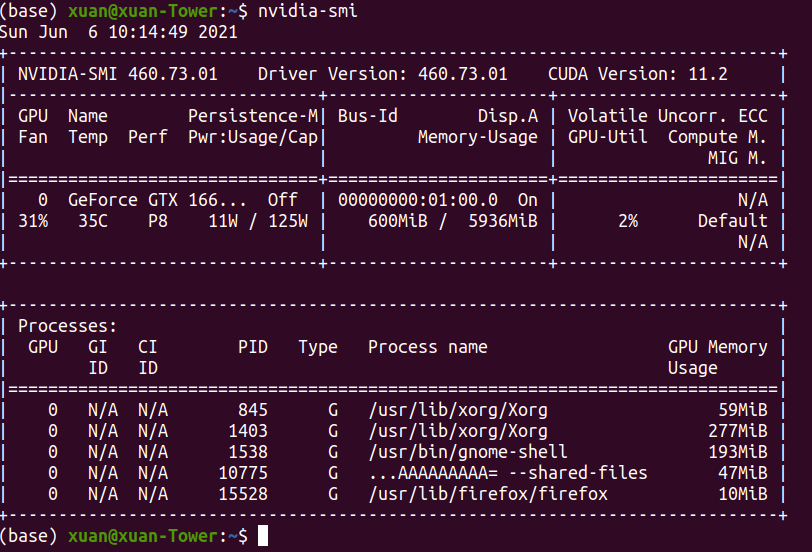
\includegraphics[width=0.8\textwidth]{pictures/nvidia-smi.png}}
\caption{英伟达显卡驱动信息}
%\label{fig:367}
\end{figure}







\chapter{软件应用}
\section{搜狗/Fcitx 中文输入法}
参考:\url{https://pinyin.sogou.com/linux/}

Fcitx 是一款不错的中文输入法。
\begin{itemize}
\item \verb|sudo apt-get install fcitx-table-wbpy|

\item System Settings $\Longrightarrow$ Language Support $\Longrightarrow$
Keyboard input method system 由默认IBus改成 fcitx

\item reboot

\item 从Ubuntu右上角顶栏的小键盘图标中打开,Configure。在 Input Method 选项下添加输入法。搜索 Pinyin 添加进去,就可以了。快捷键的设置,都在小键盘图标中。
\end{itemize}



\section{uGet下载工具}
\url{https://blog.csdn.net/u010445843/article/details/70184121}

Windows下的下载工具--迅雷,之所以下载速度快,乃是它能搜索资源、为己所用,而不是仅仅从原始地址这单一资源处下载。Ubuntu下也有类似的工具,那就是aira2。
aira2是一个命令行下载工具,可以配合其他图形界面的下载软件使用。我用的是uget+aria2。uget本身是一个小巧实用的多线程下载工具,加上aria2作为插件,下载速度有明显提高。

(1)uGet主页:\url{http://ugetdm.com}。Ubuntu安装:\\
\verb|sudo add-apt-repository ppa:plushuang-tw/uget-stable|\\
\verb|sudo apt update|\\
\verb|sudo apt install uget|

(2)安装aria2插件:\verb|sudo apt install aria2|

(3)打开uGet在设置中找到插件,选择aria2。注意,重启生效。





\section{文本编辑软件}
\subsection{gedit}
。。。


\subsection{Sublime}
官网有很详细的安装说明:
\url{https://www.sublimetext.com/download}

\subsection{Vim}
安装:\verb|sudo apt install vim|

\subsubsection{常用配置}
\begin{verbatim}
set nu
set fileencodings=utf-8,gbk,default,latin1
set encoding=utf-8
let $LANG="zh_CN.UTF-8"
\end{verbatim}


\subsubsection{一般模式(命令模式)}
\paragraph{打开文件、保存、关闭文件}
\begin{itemize}
\item vi filename :打开filename文件
\item w :保存文件
\item w vpser.net :保存至vpser.net文件
\item q :退出编辑器,如果文件已修改则用下面的命令
\item q! :退出编辑器,且不保存
\item wq :退出编辑器,且保存文件
\end{itemize}


\paragraph{常用光标移动命令}
\begin{itemize}
\item {\color{red}注意区分大小写}
\item h:左;j:下;k:上;l:右;这很符合书写习惯,用下就知道了
\item n<hjkl>移动相应字符
\item 0:零,移动到这一行最前面的字符处
\item \$ :移动到这一行最后面的字符处
\item G:移动到文件的最后一行
\item nG:n表示数字,移动到这个文件的第n行
\item n<Enter>:n表示数字,光标向下移动n行,等效于nj
\item 空格键:向右
\item Backspace :向左
\item Enter :移动到下一行首
\item - :移动到上一行首
\end{itemize}


\paragraph{搜索与替换}
\begin{itemize}
\item /word:从光标位置开始,向下搜索一个名为“word”的字符
\item ?word:从光标位置开始,向上搜索一个名为“word”的字符
\item n:表示“next”
\item N:表示“previous”
\item \%s/word1/word2/g:表示将word1替换为word2,g表示全局替换
\item \%s/word1/word2/gc:其中多的一个c表示替换之前有个用户提示,需要确认
\end{itemize}


\paragraph{删除、复制与粘贴}
\begin{itemize}
\item x,X:小写x表示向后删除字符;大写X表示向前删除字符
\item nx:表示向后删除n个字符
\item dd:表示删除光标所在的整行
\item ndd:表示包括光标所在行向下删除n行
\item d1G:表示删除当前行到第1行所有的数据
\item dG:删除光标所在位置到最后一行所有的数据
\item yy:复制光标所在的一整行,也可以用 ayy 复制,a 为缓冲区,a也可以替换为a到z的任意字母,可以完成多个复制任务。
\item nyy:n表示数字,复制光标所在的向下n行,也可以用 anyy 复制,a 为缓冲区,a也可以替换为a到z的任意字母,可以完成多个复制任务。
\item p,P:p将已复制的数据粘贴到光标下一行,P相反,如果使用了前面的自定义缓冲区,建议使用“ap”或“aP”进行粘贴。
\item J:将光标所在的行与下一行结合在一起
\item u,U:小写u撤销上一步操作,大写U撤销对当前行的所有操作
\item Ctrl+r:重做上一个操作,恢复
\item .:重复前一个动作
\item :复制单个字符:首先进入正常模式(一般模式)然后按v,进入visual方式,然后就可以移动方向键选中文本,然后按y,就拷贝完成。
\end{itemize}


\subsubsection{编辑模式}
\begin{itemize}
\item i,I:i从当前光标所在处插入,I从当前所在行的第一个非空格处开始插入
\item a,A:a从当前光标所在处下一个字符开始插入,a从当前所在行的最后一个非空格处开始插入。A是从所在行尾插入。
\item o,O:o在当前光标所在的下一行插入一个行行,O相反
\item r,R:r会替换光标所在的那一个字符,R会一直替换光标所在的字符
\item J :合并光标所在行及下一行为一行(命令模式)
\end{itemize}



\subsubsection{vim中使用系统粘贴板}
%\url{http://www.linuxsir.org/bbs/thread344622.html}
用vim这么久了,始终也不知道怎么在vim中使用系统粘贴板,通常要在网上复制一段代码都是先gedit打开文件,中键粘贴后关闭,然后再用 vim打开编辑,真的不爽;上次论坛上有人问到了怎么在vim中使用系统粘贴板,印象里回复很多,有好几页的回复却没有解决问题,今天实在受不了了又在网上找办法,竟意外地找到了,贴出来分享一下。 

如果只是想使用系统粘贴板的话直接在输入模式按Shift+Inset就可以了,下面讲一下vim的粘贴板的基础知识,有兴趣的可以看看,应该会有所收获的。 
vim帮助文档里与粘贴板有关的内容如下: 

1. vim有12个粘贴板,分别是0、1、2、...、9、a、“、+;用:reg命令可以查看各个粘贴板里的内容。在vim中简单用y只是复制到“(双引号)粘贴板里,同样用p粘贴的也是这个粘贴板里的内容; 

2. 要将vim的内容复制到某个粘贴板,需要退出编辑模式,进入正常模式后,选择要复制的内容,然后按"Ny完成复制,其中N为粘贴板号(注意是按一下双引号然后按粘贴板号最后按y),例如要把内容复制到粘贴板a,选中内容后按"ay就可以了,有两点需要说明一下: 
* “号粘贴板(临时粘贴板)比较特殊,直接按y就复制到这个粘贴板中了,直接按p就粘贴这个粘贴板中的内容; 
* +号粘贴板是系统粘贴板,用"+y将内容复制到该粘贴板后可以使用Ctrl+V将其粘贴到其他文档(如firefox、gedit)中,同理,要把在其他地方用Ctrl+C或右键复制的内容复制到vim中,需要在正常模式下按"+p; 

3. 要将vim某个粘贴板里的内容粘贴进来,需要退出编辑模式,在正常模式按"Np,其中N为粘贴板号,如上所述,可以按"5p将5号粘贴板里的内容粘贴进来,也可以按"+p将系统全局粘贴板里的内容粘贴进来。 






\section{Gnuplot 绘图工具}
这是自己早期经常用的绘图工具,现在已经完全用Python实现,不再使用。

\subsection{安装}
(一)

注意不要直接安装,即\verb*|sudo apt-get install gnuplot|,通常缺少一个外界的库,容易造成terminal set to unknown错误,进而不能显示绘制图片。采用以下命令安装:

\verb*|sudo apt-get install gnuplot-x11|

或者分两步安装

\verb*|sudo apt-get install libx11-dev|

\verb*|sudo apt-get install gnuplot|



(二)源代码编译安装
\begin{itemize}
\item 先执行\verb*|sudo apt-get install libx11-dev|  安装x11,否则不能显示图形!\\
若不安装,则会出现,在终端下输入gnuplot后显示terminal set to unknown。

\item 去官网下载gnuplot版本并解压

\item \verb*|su root|

\item 切换到gnuplot所在目录

\item 配置\verb*|./configure|

\item 编译 make

\item  make install

\item 运行:在终端输入 gnuplot 就行了

\item 例子: plot sin(x)
\end{itemize}



\subsection{文件设置}
\subsubsection{设置数据分隔符}
%http://blog.csdn.net/liyuanbhu/article/details/8516417
\begin{verbatim}
set datafile separator ","
#设置gnuplot读取逗号分隔的数据文件
\end{verbatim}

有时,我们的数据文件中各个数据之间是用逗号作为分隔符的,比如标准的以“CSV”(Comma-Separated Values)为后缀的数据文件。如果在逗号之后没有空格分隔,默认情况下gnuplot是无法直接读取的。这时可以有两种方案,第一种是提前处理一下数据文件,比如将逗号替换为空格,随便一个文本处理软件都能很轻松的做这种替换。但是有时我们有很多这样的数据文件,每个都这样处理一下也挺麻烦的。第二种方法就是在gnuplot中给出文件分隔符的信息,让gnuplot能够读懂我们的文件。

例如:

\verb*|Plot 'sample.csv' using 1:2|

gnuplot 会抱怨说:
\begin{verbatim}
gnuplot> plot 'sample.csv' using 1:2
                                   ^
         warning: Skipping data file with no valid points
                                    ^
         x range is invalid
\end{verbatim}

正确的方法是这样的:

\verb*|plot 'sample.csv' using 1:2 "%lf,%lf"|

格式字符串的格式与C语言中scanf的格式字符串是类似的,实际上gnuplot就是用的scanf函数来读取数据。\verb|%lf| 
表示按照 double型浮点数类型来读取。需要注意的是gnuplot的格式化字符串不支持\verb|%lf| 。
gnuplot的格式化字符串还有很多的用法,这里就不多介绍了,有兴趣的可以参考帮助文档相关章节。

更一般的参考说明文档
\begin{verbatim}
Set datafile separator
The command set datafile separator tells gnuplot that data fields in subsequent input files are separated
by a specific character rather than by whitespace. The most common use is to read in csv (comma-separated
value) files written by spreadsheet or database programs. By default data fields are separated by whitespace.
Syntax:
set datafile separator {whitespace | tab | comma | "<chars>"}
Examples:
# Input file contains tab-separated fields
set datafile separator "\t"
# Input file contains comma-separated values fields
set datafile separator comma
# Input file contains fields separated by either * or |
set datafile separator "*|"
\end{verbatim}


\subsubsection{重命名数据文件}
\begin{verbatim}
datafile = "FMO-sink-initial1.ods"
#将数据文件命名为“datafile”,方便调用
\end{verbatim}



\subsection{图片设置}
\subsubsection{设置输出图片格式和名称}
\begin{verbatim}
set term post eps color enh solid
#设置输出图片格式
set output "FMO-sink-initial1.eps"
#设置输出图片名称
\end{verbatim}

其他图片格式的,有
\begin{itemize}
\item PS格式:
彩色(推荐使用):
\begin{verbatim}
set term postscript enhanced color
set output "*.ps"
\end{verbatim}
另:(未测)
\begin{verbatim}
set term postscript landscape
set output "*.ps"
\end{verbatim}

\item EPS格式:
黑白(曲线类型控制未知):
\begin{verbatim}
set term postscript eps enhanced
set output "*.eps"
\end{verbatim}
忘了是啥:
\begin{verbatim}
set term post eps color solid enh
set output "*.eps"
\end{verbatim}

\item PNG格式:
\begin{verbatim}
set terminal png size 1500,1000 enhanced font "Helvetica,20"
set output '*.png'
\end{verbatim}

\item PDF格式需要装有ps2pdf,然后:
\begin{verbatim}
set term postscript enhanced color
set output "| ps2pdf - *.pdf"
\end{verbatim}

注:关于pdf图片,输出后周围的大片空白可以在终端中使用如下命令去除:
pdfcrop *.pdf
会生成一个新文件: *-crop.pdf
使用此pdf文件在Latex等处都将十分整洁方便,妈妈再也不用担心我的图片了。
\end{itemize}


\subsubsection{设置图片/字体大小}
\begin{verbatim}
set size 1.0,1.0
#设置图片大小
\end{verbatim}
字体大小设置比较复杂,此命令是按比例缩放图片大小,字体大小不变,相当于字体相对变大。


\subsubsection{设置图片标题}
 设置/取消命名(位于图上方)
 \begin{verbatim}
set title "figurename""
unset title
\end{verbatim}
注:在多图设置(见8小节)中,命名命令对其后所有图生效,要在每个图中重新命名。之后不需要命名时要记得取消。


\subsubsection{设置图注}
\begin{enumerate}
\item 图注在图中的位置:
\verb*|set key left/right top/bottom/center|

\item 图注增加/取消外框:\verb*|set/unset key box|

\item 图注间距:\verb*|set key spacing 1.5|

\item 图注位于图外:\verb*|set key lmargin/rmargin/tmargin/bmargin(below)|

\item 取消图注:\verb*|unset key|
\end{enumerate}

图注设置参数一览:
\begin{verbatim}
set key {on|off} {default}
             {{inside | outside} | {lmargin | rmargin | tmargin | bmargin}
               | {at <position>}}
             {left | right | center} {top | bottom | center}
             {vertical | horizontal} {Left | Right}
             {{no}reverse} {{no}invert}
             {samplen <sample_length>} {spacing <vertical_spacing>}
             {width <width_increment>}
             {height <height_increment>}
             {{no}autotitle {columnheader}}
             {title "<text>"} {{no}enhanced}
             {{no}box { {linestyle | ls <line_style>}
                        | {linetype | lt <line_type>}
                          {linewidth | lw <line_width>}}}
     unset key
     show key
\end{verbatim}



\subsection{坐标轴设置}
\subsubsection{设置/取消坐标名称}
 \begin{verbatim}
set xlabel/ylabel "name"
unset xlabel/ylabel
\end{verbatim}


\subsubsection{设置坐标轴范围}
\begin{itemize}
\item 设置给定坐标轴范围\\
\verb|set xrange/yrange [1:100]|

\item 设置负向坐标
\verb|set xrange/yrange [100:1]|

\item 只设置一端坐标(另一端将自动调整)\\
\verb|set xrange/yrange [:100]|

\item 恢复自动坐标轴范围(此时人工给定设置依然保留)\\
\verb|set auto x/y|

\item  恢复给定坐标轴范围\\
\verb|set noauto x/y|
\end{itemize}

注:坐标轴范围,可以不设置,自动判断



\subsubsection{设置坐标轴标识}
\begin{itemize}
\item 设置坐标轴最大间隔(显示数值)\\
\verb|set xtics/ytics 0.5|

\item 设置坐标轴小间隔\\
\verb|set mxtics/mytics 2|\\
说明:将每个大间隔平分为2份

\item 设置坐标轴刻度的精度\\
\verb|set xtics format "%.2f"|\\
\verb|set ytics format "%.0f"|\\
说明:“\%.2f”指的是浮点型、精确到小数点后两位

\item 设置标识文本显示倾斜度\\
\verb|set xtics rotate by -45|\\
说明:标识右倾45度

\item 设置指数坐标轴\\
\verb|set log x/y|\\
\verb|set xtics 1.5|\\
说明:设置指数坐标轴的间隔时,数字代表10的指数(待明)。注意此时坐标的值域必须大于0。

\item 移动坐标标记\\
\verb|set x/ytics [out] offset 1,1|\\
“1,1” 为对应的移动向量的x,y值。
\end{itemize}



\subsection{代码示例}
\subsubsection{一维绘图图}
\lstinputlisting[language=gnuplot]{program/gnuplot/plot_1d.sh}
效果如下:
\begin{figure}[htb]
\centering
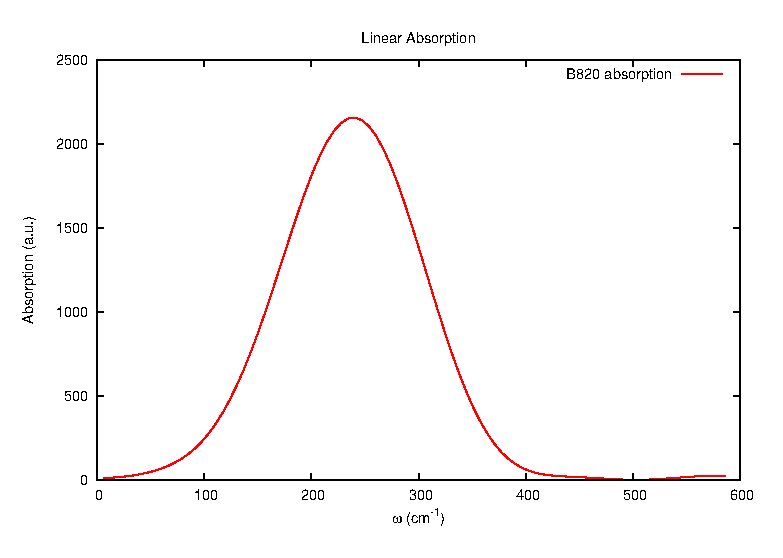
\includegraphics[width=0.7\textwidth]{program/gnuplot/diagonal.eps}
%\caption{精确解、欧拉法解、改进欧拉法解}
%\label{fig:by:table}
\end{figure}



\subsubsection{二维三维绘图}
给数据加入空白行Shell脚本:
\lstinputlisting[language=sh]{program/gnuplot/addblanks.awk}
二维等高图代码:
\lstinputlisting[language=gnuplot]{program/gnuplot/2d_contour.sh}
三维绘图代码:
\begin{lstlisting}[language=gnuplot]
#==================Pm3d绘图====================#
unset key
#pm3d绘图时,NxM的数据只能画出(N-1)x(M-1)的图像
set pm3d
#用色彩来表示不同的z值,palette-mapped 3d.
set palette rgbformulae 22,13,-31
#设置色板
replot

set pm3d at bs
#色彩图除了画在曲面上,还可以画在底部或顶部。b,s,t 三个字母分别代表底部、曲面和顶部,at 之后可以是任一个字母,也可是三个字母的任意组合。
replot
#splot datafile with lines

set pm3d map
#从上往下看数据
set size square
replot


#=================Image绘图===================#
set size square
plot datafile with image
#Image绘图与Pm3d绘图这两种方式无法简单判断优劣,只能根据实际需要选择。当像素比较多而数据又比较平滑的时候,其实两者差别不大。
\end{lstlisting}


效果如下:

%\begin{figure}[htb]
%\centering

\includegraphics[width=0.4\textwidth]{program/gnuplot/re_rp1.eps}
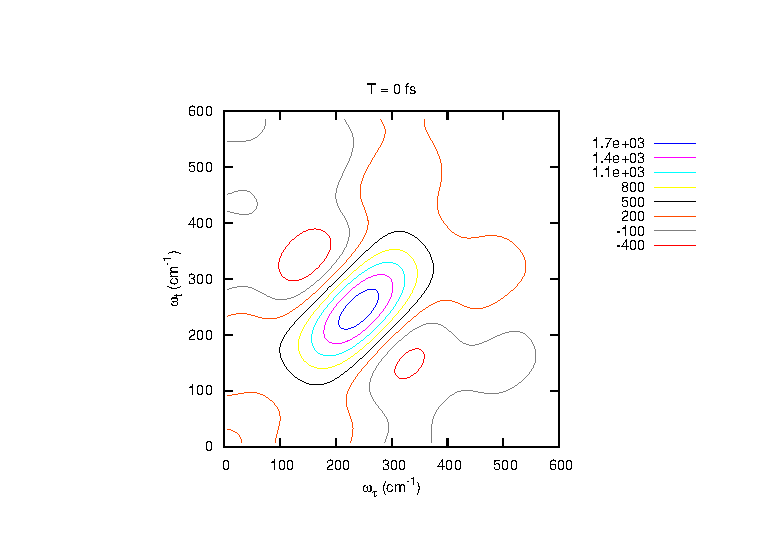
\includegraphics[width=0.4\textwidth]{program/gnuplot/re_rp2.eps}

\includegraphics[width=0.7\textwidth]{program/gnuplot/re_rp3.eps}


\includegraphics[width=0.7\textwidth]{program/gnuplot/re_rp4.eps}
%\caption{精确解、欧拉法解、改进欧拉法解}
%\label{fig:by:table}
%\end{figure}







\newpage
\section{Fortran 编译器}
\subsection{Intel visual Fortran}
\url{https://software.intel.com/content/www/us/en/develop/articles/intel-visual-fortran-compiler-190-for-windows-release-notes-for-intel-parallel-studio-xe-2019.html}

\subsection{Intel Fortran}
\subsubsection{编译器的获取——完全免费开放了}
开发工具合集地址:\url{https://software.intel.com/content/www/us/en/develop/articles/free-intel-software-developer-tools.html}

各个组分地址:\url{https://software.intel.com/content/www/us/en/develop/articles/oneapi-standalone-components.html}

Fortran编译器地址:\url{https://software.intel.com/content/www/us/en/develop/articles/oneapi-standalone-components.html#fortran}


\subsubsection{编译器的安装}
参考:\url{https://software.intel.com/content/www/us/en/develop/documentation/get-started-with-intel-oneapi-base-linux/top/before-you-begin.html}

\begin{itemize}
\item (可能需要)预装Java运行环境;
\item  预装suite of GNU development tools:\\
\verb*|sudo apt -y install cmake pkg-config build-essential|;
\item 下载的编译器文件为:\verb|l_fortran-compiler_p_2021.1.2.62_offline.sh|,右键点击属性勾选为可执行文件;
\item \verb|sudo ./l_fortran-compiler_p_2021.1.2.62_offline.sh|;
\item 安装界面为图形化界面,采用默认安装路径;
\item 路径(环境)设置:在\verb*|~/.bashrc|中加入:\\
\verb|source /opt/intel/oneapi/setvars.sh|\\
或\\
\verb|source /opt/intel/oneapi/compiler/2021.1.2/env/vars.sh|(不同的版本,路径或者名称不一样)
\item 注销生效
\item 查看是否安装成功:\verb|which ifort|,如果成功会显示编译器路径。
\end{itemize}


\subsection{常见报错}
(1)forrtl: severe (174): SIGSEGV, segmentation fault occurred

在Linux下写程序的时候,如果程序比较大,经常会遇到“段错误”(segmentation fault)这样的问题,这主要就是由于Linux系统初始的堆栈大小(stack size)太小的缘故,一般为10M。

\#set unlimited stack size:ulimit -s unlimited

\#check stack size:ulimit -a

可以在 .bashrc 和 /root/.bashrc 中添加



\section{Python开发环境}
Anaconda官网下载,建议非root直接安装,不然不太方便。


\section{SSH远程登录服务器}
SSH 为 Secure Shell 的缩写,由 IETF 的网络工作小组(Network Working Group)所制定;SSH 为建立在应用层和传输层基础上的安全协议。SSH 是目前较可靠,专为远程登录会话和其他网络服务提供安全性的协议。利用 SSH 协议可以有效防止远程管理过程中的信息泄露问题。SSH最初是UNIX系统上的一个程序,后来又迅速扩展到其他操作平台。SSH在正确使用时可弥补网络中的漏洞。SSH客户端适用于多种平台。几乎所有UNIX平台—包括HP-UX、Linux、AIX、Solaris、Digital UNIX、Irix,以及其他平台,都可运行SSH。

SSH分为客户端和服务端。服务端是一个守护进程,一般是sshd进程,在后台运行并响应来自客户端的请求。提供了对远程请求的处理,一般包括公共密钥认证、密钥交换、对称密钥加密和非安全连接。
客户端一般是ssh进程,另外还包含scp、slogin、sftp等其他进程。客户端不是必须的。

工作机制:
\begin{enumerate}
\item 客户端发送一个连接请求到远程服务端;
\item 服务端检查申请的包和IP地址,再发生密钥给SSH客户端;
\item 客户端再将密钥发回服务端,自此建立连接。
\end{enumerate}


\subsection{服务端}
1、安装服务器

\verb|sudo apt-get install openssh-server|

2、查看服务器

\verb{ps -e|grep ssh{

如果看到sshd则表示sshserver已经启动,如果只有ssh-agent,则表示没有启动。

3、启动服务器
\begin{itemize}
\item \verb|sudo service ssh start|
\item \verb|sudo /etc/init.d/ssh stop| ,\#停止
\item \verb|sudo /etc/init.d/ssh start|,\#启动
\item \verb|sudo /etc/init.d/ssh restart| ,\#重启
\end{itemize}

4、配置

修改配置文件:\verb|sudo gedit /etc/ssh/sshd_config|,并重启服务。
\begin{itemize}
\item  把配置文件中的“PermitRootLogin without-password"加一个”\#"号,把它注释掉;再增加一句“PermitRootLogin yes";保存。
\item ssh默认端口是22,Port 20,需要的话,自行修改。
\item ssh默认配置是允许root登录的,可以修改配置表禁止其登录:PermitRootLogin no
\end{itemize}

5、登录

\verb|ssh 服务器用户名@服务器地址|,例如:\verb|ssh sm06@10.125.6.30|


\subsection{用户端}
遇到更换服务器的情形,使用如下命令删除原密钥。

\verb|ssh-keygen -f "/home/xuanleng/.ssh/known_hosts" -R 159.226.204.95|

冒号内为known\_hosts文件全路径,“159.226.204.95”为要删除的服务端地址。



\subsection{远程文件传输}
\subsubsection{scp}
在Linux下一般通过scp命令在本地机和服务器(超算)间传输文件。所以使用时一定要明确是在本地终端使用还是在超算终端使用。

1、从服务器上下载文件

(1)从本地终端下载

\verb*|scp username@servername:/path/filename .|

其意思按字面理解,其中“.”表示当前目录。例如,
\begin{verbatim*}
phileas@phileas-computer:~$ scp lengxuan@10.22.20.156:/home/lengxuan/1/sum_als.ods .
\end{verbatim*}
其中lengxuan为超算用户名,10.22.20.156为超算地址。


(2)从超算终端下载

命令反过来就是了,例如:

\verb*|[lengxuan@hpc 1]$ scp sum_als.ods phileas@10.22.21.70:/home/phileas|

其中\verb*|[lengxuan@hpc 1]|表示在超算用户lengxuan主目录下的1目录中。使用大致是这样,这样不方便用,因为对自己的IP不是很清楚。

2、上传本地文件到服务器

原理同上

3、从服务器上下载整个目录

也是分从本地终端下载和从服务器上下载两种,原理同上,和上传(下载)文件不同的是,上传(下载)目录多了一个参数,如

\verb*|scp -r root@192.168.0.101:/var/www/test  /var/www/  |

4、从本地上传目录到服务器

原理同上



\subsubsection{sftp}
sftp是Secure File Transfer Protocol的缩写,安全文件传送协议。可以为传输文件提供一种安全的加密方法。sftp 与 ftp 有着几乎一样的语法和功能。SFTP 为 SSH的一部分,是一种传输档案至 Blogger 伺服器的安全方式。其实在SSH软件包中,已经包含了一个叫作SFTP(Secure File Transfer Protocol)的安全文件传输子系统,SFTP本身没有单独的守护进程,它必须使用sshd守护进程(端口号默认是22)来完成相应的连接操作,所以从某种意义上来说,SFTP并不像一个服务器程序,而更像是一个客户端程序。SFTP同样是使用加密传输认证信息和传输的数据,所以,使用SFTP是非常安全的。但是,由于这种传输方式使用了加密/解密技术,所以传输效率比普通的FTP要低得多,如果您对网络安全性要求更高时,可以使用SFTP代替FTP。

1、终端登录

\verb|sftp 服务器用户名@服务器地址|,例如:\verb|sftp sm06@10.125.6.30|,登入成功后终端呈现出:sftp>....

2、操作

在sftp的环境下的操作就和一般ftp的操作类似了,\verb|ls|、\verb|rm|、\verb|mkdir|、\verb|dir|、\verb|pwd|,等指令都是对远端进行操作。如果要对本地操作,只需在上述的指令上加“\verb|l|”变为:\verb|lls|、\verb|lcd|、\verb|lpwd|等。

3、上传与下载

\begin{itemize}
\item 上传:put /path/filename(本地主机) /path/filename(远端主机);
\item 下载:get /path/filename(远端主机) /path/filename(本地主机)。
\end{itemize}



\subsection{解决ssh的``Write failed: Broken pipe"问题}
%本节摘自:\url{http://www.cnblogs.com/dudu/archive/2013/02/07/ssh-write-failed-broken-pipe.html}

\textbf{问题场景}

服务器环境:阿里云 Linux CentOS 主机

客户端:Mac OSX Terminal

\textbf{问题现象}

用 ssh 命令连接服务器之后,如果一段时间不操作,再次进入 Terminal 时会有一段时间没有响应,然后就出现错误提示:

\verb|Write failed: Broken pipe|

只能重新用 ssh 命令进行连接。

\textbf{解决方法}

方法一:如果您有多台服务器,不想在每台服务器上设置,只需在客户端的 \verb*|~/.ssh/| 文件夹中添加 config 文件,并添加下面的配置:

\verb*|ServerAliveInterval 60|

方法二:如果您有多个人管理服务器,不想在每个客户端进行设置,只需在服务器的 \verb*|/etc/ssh/sshd_config| 中添加如下的配置:

\verb*|ClientAliveInterval 60|

方法三:如果您只想让当前的 ssh 保持连接,可以使用以下的命令:

\verb*|$ ssh -o ServerAliveInterval=60 user@sshserver|


在linux下终端用超算也会遇到同样的问题,按上述方法解决。


\subsection{Windows客户端—Putty}
\url{https://www.putty.org}

PuTTY is an SSH and telnet client, developed originally by Simon Tatham for the Windows platform. PuTTY is open source software that is available with source code and is developed and supported by a group of volunteers.


\section{SSHFS 远程挂载文件夹}
\verb| sudo apt-get install sshfs|

\verb*|sshfs xuan@192.168.1.2:/home hpc1|
其中\verb|/home|为远程目录,\verb|hpc1|为本地空目录,用来挂载远程目录。


\section{Linux作业管理系统}
\subsection{PBS}
\begin{itemize}
\item \url{https://www.jianshu.com/p/2f6c799ca147}
\end{itemize}


PBS(Portable Batch System)最初由NASA的Ames研究中心开发,主要为了提供一个能满足异构计算网络需要的软件包,用于灵活的批处理,特别是满足高性能计算的需要,如集群系统、超级计算机和大规模并行系统。PBS的主要特点有:代码开放,免费获取;支持批处理、交互式作业和串行、多种并行作业,如MPI、PVM、HPF、MPL。PBS是功能最为齐全, 历史最悠久, 支持最广泛的本地集群调度器之一。PBS的目前包括openPBS、PBS Pro和Torque三个主要分支。 其中OpenPBS是最早的PBS系统, 目前已经没有太多后续开发;PBS pro是PBS的商业版本,功能最为丰富; Torque是Clustering公司接过了OpenPBS,并给与后续支持的一个开源版本。


\subsubsection{Ubuntu14.04安装配置Torque}
{\color{red} 很不幸!Ubuntu 18.04后兼容很不好了}
\begin{itemize}
\item \url{https://jabriffa.wordpress.com/2019/06/27/installing-grid-engine-on-ubuntu-18-04-lts/}
\item \url{https://jabriffa.wordpress.com/2015/02/11/installing-torquepbs-job-scheduler-on-ubuntu-14-04-lts/}
\end{itemize}


[转]\url{http://blog.sina.com.cn/s/blog_4a0a8b5d0102v2p1.html}

其实Ubuntu有编译好的Torque,只需要安装 torque-server torque-mom torque-scheduler,再加些配置即可。但是发现它弄得scp秘钥有问题,配置了半天rsa秘钥也没有解决日志移位的问题。所以还是自己编译吧!

\textbf{1、下载Torque源代码}\\
\verb|git clone https://github.com/adaptivecomputing/torque.git -b 6.1.3 6.1.3|\\
通过修改参数,下载最新版本。

\textbf{2、解压并编译}

\begin{lstlisting}[language=sh]
tar -xzvf torque-4.1.7.tar.gz

cd torque-4.1.7

./autogen.sh

./configure --prefix=/usr/local/torque
\end{lstlisting}

提示缺少 openssl-dev和 libxml2-dev之类的,补上它们……

configure: error: TORQUE needs lib openssl-devel in order to build

输入 sudo apt-get install libssl-dev

configure: error: TORQUE needs lib libxml2-devel in order to build

输入 sudo apt-get install libxml2-dev

……

1)出现问题
\begin{verbatim}
configure: error: TORQUE needs libxml2-devel in order to build
\end{verbatim}

解决:\\
\verb|./configure LDFLAGS="-L/home/xuanleng/anaconda3/lib" --prefix=/usr/local/torque|

2)出现问题
\begin{verbatim}
libtool: Version mismatch error. This is libtool 2.2.6 Debian-2.2.6a-4, but the
libtool: definition of this LT_INIT comes from libtool 2.2.6b.
libtool: You should recreate aclocal.m4 with macros from libtool 2.2.6 Debian-2.2.6a-4
libtool: and run autoconf again.
make[2]: *** [wktools4] Error 63
make[2]: Target `all' not remade because of errors.
make[1]: *** [all-recursive] Error 1
make: *** [all] Error 2
*** Exited with status: 2 ***
\end{verbatim}
解决:\\
\verb|autoreconf -fi  configure.ac |



直至 ./configure --prefix=/usr/local/torque没有提示缺少库,ready to make为止。

像这样提示:
\begin{verbatim}
Building components: server=yes mom=yes clients=yes
                     gui=no drmaa=no pam=no
PBS Machine type    : linux
Remote copy         : /usr/bin/scp -rpB
PBS home            : /var/spool/torque
Default server      : rccm
Unix Domain sockets :
Linux cpusets       : no
Tcl                 : disabled
Tk                  : disabled
\end{verbatim}

\begin{lstlisting}[language=sh]
make

sudo make install
\end{lstlisting}

\textbf{3. 设置环境变量并刷新}

刷新环境变量需要注意时效性,如果root或sudoer退出终端,在没有重启机器的前提下,那么还是要刷新下的,不然可能会提示没有trqauthd之类的错误。
\begin{lstlisting}[language=sh]
sudo vi /etc/profile
\end{lstlisting}
添加
\begin{lstlisting}[language=sh]
#Torque
export PATH=/usr/local/torque/bin:/usr/local/torque/sbin:$PATH
\end{lstlisting}
刷新环境变量
\begin{lstlisting}[language=sh]
sudo -s
source /etc/profile
\end{lstlisting}

\textbf{4.、安装}

需管理员权限,仍然在 torque-4.1.7 文件夹下。
\begin{lstlisting}[language=sh]
sudo ./torque.setup root
\end{lstlisting}
如果出现:
\begin{verbatim}
mxio@Node1:~/Downloads/torque-4.1.7$ sudo ./torque.setup root
./torque.setup: 1: ./torque.setup: trqauthd: not found
trqauthd failed to start!!! exiting setup 
\end{verbatim}
错误,那么请检查第三步并刷新source /etc/profile。

出现类似下面的成功:
\begin{verbatim}
pbs_server port is: 15001
trqauthd daemonized - port 15005
trqauthd successfully started
initializing TORQUE (admin: root@Node1)
You have selected to start pbs_server in create mode.
If the server database exists it will be overwritten.
do you wish to continue y/(n)?y
root       495     1  1 17:40 ?        00:00:00 pbs_server -t create
Max open servers: 9
Max open servers: 9
\end{verbatim}


\textbf{5、配置}

需管理员权限
\begin{lstlisting}[language=sh]
sudo -s
\end{lstlisting}
查看计算机名
\begin{lstlisting}[language=sh]
hostname
\end{lstlisting}
输出 Node1 (服务器计算机名)
\begin{lstlisting}[language=sh]
vi /etc/hosts
\end{lstlisting}
 将计算机名添加进hosts,我选择注释掉127.0.1.1 Node1,改成:
 \begin{verbatim}
127.0.0.1        Node1 localhost
#127.0.1.1      Node1
\end{verbatim}
进入torque主目录进行环境变量设置:
\begin{lstlisting}[language=sh]
cd /var/spool/torque
vi server_priv/nodes
\end{lstlisting}
添加:
 \begin{verbatim}
Node1 np=32
\end{verbatim}
即计算机名和CPU数目,这个视具体情况而定。
\begin{lstlisting}[language=sh]
vi mom_priv/config
\end{lstlisting}
添加:
\begin{verbatim}
$pbs_server = 127.0.0.1
\end{verbatim}
\begin{lstlisting}[language=sh]
vi server_name
\end{lstlisting}
添加:
\begin{verbatim}
Node1
\end{verbatim}


\textbf{6、启动client daemon}

\verb|pbs_mom|

\textbf{7、重启pbs server daemon}
\begin{verbatim}
qterm
pbs_server
\end{verbatim}

\textbf{8、启动scheduler daemon}

\verb|pbs_sched|

\textbf{9、检查服务是否正确启动}
\begin{verbatim}
ps -aux | grep pbs #check all is running
qstat -q #check the presence of the queue
qmgr -c 'p s' #check server & queue settings
pbsnodes -a  #check if the nodes are listed and u
\end{verbatim}

\textbf{10、配置列队}
\begin{verbatim}
qmgr -c "set queue batch resources_default.walltime = 360:00:00"
qmgr -c "set server query_other_jobs = True"
qmgr -c "set queue batch resources_max.ncpus=32"
\end{verbatim}

\textbf{11. 测试列队}

首先退出root
\begin{lstlisting}[language=sh]
exit
\end{lstlisting}
\begin{lstlisting}[language=sh]
source /etc/profile
echo "sleep 30" | qsub
qstat
\end{lstlisting}

\textbf{12、配置开启启动}

cd到torque-2.4.6/contrib/init.d目录下
\begin{lstlisting}[language=sh]
sudo -s
cp debian.pbs_mom /etc/init.d/pbs_mom && update-rc.d pbs_mom defaults
cp debian.pbs_server /etc/init.d/pbs_server && update-rc.d pbs_server defaults
cp debian.pbs_sched /etc/init.d/pbs_sched && update-rc.d pbs_sched defaults
cp debian.trqauthd /etc/init.d/trqauthd && update-rc.d trqauthd defaults
\end{lstlisting}
注,请检查DAEMON是否为\verb|/usr/local/torque/sbin/$NAME|,不是的话请修改。

\textbf{13、重启计算机}
\begin{lstlisting}[language=sh]
echo "sleep 30" | qsub
qstat
\end{lstlisting}
输出:
\begin{verbatim}
Job ID                    Name             User            Time Use S Queue
------------------------- ---------------- --------------- -------- - -----
2.Node1                    STDIN            mxio                   0 Q batch
\end{verbatim}
成功搞定。



\subsubsection{重要说明}
第二次安装开机自起没有配置成功。需要手动开启服务。
进入root权限,依次输入如下命令:

\verb|service pbs_server restart|

\verb|service pbs_mom server restart|

\verb|pbs_sched|

\verb|trqauthd|


\subsubsection{PBS命令}
PBS 提供4 条命令用于作业管理。

(1) qsub 命令—用于提交作业脚本

命令格式:
\begin{verbatim}
qsub [-a date_time] [-c interval] [-C directive_prefix]
[-e path] [-I] [-j join] [-k keep] [-l resource_list] [-m mail_options]
[-M user_list][-N name] [-o path] [-p priority] [-q destination] [-r c]
[-S path_list] [-u user_list][-v variable_list] [-V]
[-W additional_attributes] [-z]
[script]
\end{verbatim}
参数说明:因为所采用的选项一般放在pbs 脚本中提交,所以具体见PBS 脚本选项。

例: qsub aaa.pbs 提交某作业,系统将产生一个作业号

(2) qstat 命令—用于查询作业状态信息

命令格式:
\verb*|qatat [-f][-a][-i] [-n][-s] [-R] [-Q][-q][-B][-u]|

参数说明:
\begin{itemize}
\item -f jobid 列出指定作业的信息
\item -a 列出系统所有作业
\item -i 列出不在运行的作业
\item -n 列出分配给此作业的结点
\item -s 列出队列管理员与scheduler 所提供的建议
\item -R 列出磁盘预留信息
\item -Q 操作符是destination id,指明请求的是队列状态
\item -q 列出队列状态,并以alternative 形式显示
\item -au userid 列出指定用户的所有作业
\item -B 列出PBS Server 信息
\item -r 列出所有正在运行的作业
\item -Qf queue 列出指定队列的信息
\item -u 若操作符为作业号,则列出其状态。
\end{itemize}

若操作符为destination id,则列出运行在其上的属于user\_list 中用户的作业状态。

例:qstat -f 211 查询作业号为211 的作业的具体信息。


(3) qdel 命令—用于删除已提交的作业

命令格式:

\verb*|qdel [-W 间隔时间] 作业号|

命令行参数:

例:qdel -W 15 211 

15 秒后删除作业号为211 的作业


(4) qmgr 命令—用于队列管理


qmgr -c "create queue batch queue\_type=execution"

qmgr -c "set queue batch started=true"

qmgr -c "set queue batch enabled=true"

qmgr -c "set queue batch resources\_default.nodes=1"

qmgr -c "set queue batch resources\_default.walltime=3600"

qmgr -c "set server default\_queue=batch"



\subsubsection{PBS 脚本文件}
PBS 脚本文件由脚本选项和运行脚本两部分组成。

(1) PBS 作业脚本选项 (若无-C 选项,则每项前面加‘\#PBS’)
\begin{itemize}
\item -a date\_time : date\_time 格式为:[[[[CC]YY]MM]DD]hhmm[.SS]
表示经过date\_time 时间后作业才可以运行。

\item -c interval : 定义作业的检查点间隔,如果机器不支持检查点,则忽略此选项。

\item -C directive\_prefix :在脚本文件中以directive\_prefix 开头的行解释为qsub 的命
令选项。(若无此选项,则默认为’\#PBS’ )

\item -e path :将标准错误信息重定向到path

\item -I :以交互方式运行

\item -j join :将标准输出信息与标准错误信息合并到一个文件join 中去。

\item  -k keep :定义在执行结点上保留标准输出和标准错误信息中的哪个文件。
keep 为o 表示保留前者,e 表示后者,oe 或eo 表示二者都保留,n 表示皆不保留。若忽略此选项,二者都不保留。

\item -l resource\_list : 定义资源列表。以下为几个常用的资源种类。
	\begin{itemize}
	\item  cput=N : 请求N 秒的CPU 时间; N 也可以是hh:mm:ss 的形式。	
	
	\item mem=N[K|M|G][B|W]:请求N {kilo|mega|giga}{bytes|words} 大小的内存。
	
	\item nodes=N:ppn=M :请求N 个结点,每个结点M 个处理器。
	\end{itemize}

\item -m mail\_options :mail\_option 为a:作业abort 时给用户发信;为b:作业开始运行发信;为e:
作业结束运行时发信。若无此选项,默认为a。

\item -M user\_list : 定义有关此作业的mail 发给哪些用户。

\item -N name : 作业名,限15 个字符,首字符为字母,无空格。

\item -o path : 重定向标准输出到path。

\item -p priority : 任务优先级,整数,[-1024,1023],若无定义则为0。

\item -q destination : destination 有三种形式: queue , @server,queue@server。

\item -r y|n : 指明作业是否可运行,y 为可运行,n 为不可运行。

\item -S shell : 指明执行运行脚本所用的shell,须包含全路径。

\item -u user\_list : 定义作业将在运行结点上以哪个用户名来运行。

\item -v variable\_list : 定义export 到本作业的环境变量的扩展列表。

\item -V : 表明qsub 命令的所有环境变量都export 到此作业。

\item -W additional\_attributes : 作业的其它属性。

\item -z : 指明qsub 命令提交作业后,不在终端显示作业号。
\end{itemize}


(2) 运行脚本同LINUX 下一般的运行脚本文件。
[注]:脚本文件中的mpirun\_rsh 命令行中的节点列表文件要用环境变量表示
\$PBS\_NODEFILE,这个环境变量表示由pbs 自动分配给作业的节点列表;
节点数为命令行中指定的进程数。
格式如下:
mpirun\_rsh –np 进程数 –hostfile \$PBS\_NODEFILE 可执行程序名



\subsubsection{设置最大队列数}
\begin{verbatim}
set value: max_running
# qmgr
Max open servers: 4
Qmgr: set queue sort max_running = 20
Qmgr: print server
.................
Qmgr: quit
check new setting:
# qmgr -c "print server" | grep max_run
set queue short max_running = 20
set queue long max_running = 20
set queue infinite max_running = 20
set queue cert max_running = 20
\end{verbatim}

\verb|qmgr -c "set queue batch max_running=20"|



\subsection{LSF}
\begin{itemize}
\item \url{https://en.wikipedia.org/wiki/Platform_LSF}
\item \url{https://www.jianshu.com/p/601ca9f33b31}
\end{itemize}


Platform Load Sharing Facility (or simply LSF) is a workload management platform, job scheduler, for distributed high performance computing. It can be used to execute batch jobs on networked Unix and Windows systems on many different architectures.[1][2] LSF was based on the Utopia research project at the University of Toronto.[3]

In 2007, Platform released Platform Lava, which is a simplified version of LSF based on an old version of LSF release, licensed under GNU General Public License v2.[4] The project was discontinued in 2011, succeeded by OpenLava.

In January, 2012, Platform Computing was acquired by IBM.[5]


\url{https://www.ibm.com/support/knowledgecenter/en/SSWRJV/product_welcome_spectrum_lsf.html}



\subsubsection{常用命令}
\begin{itemize}
\item bhosts
\item bjobs -u all, bjobs -l
\item bqueues
\end{itemize}




\subsection{Slurm}
\begin{itemize}
\item \url{https://tkainrad.dev/posts/copy-paste-ready-instructions-to-set-up-1-node-clusters/}
\item \url{https://www.schedmd.com/}
\item \url{https://slurm.schedmd.com/quickstart.html}
\item \url{https://www.jianshu.com/p/e560b19dbd3e}
\item \url{https://blog.csdn.net/cuxiong8996/article/details/107154425}
\end{itemize}


\subsubsection{单机Slurm安装}




\subsubsection{启动Slurm}
要启动SLURM,只需使用/etc/init.d/slurm中定义的管理脚本。 该脚本接受start , stop , restart和startclean (以忽略所有先前保存的状态)。 使用此方法启动SLURM会导致slurmctld守护程序(以及在此简单配置中的节点上的slurmd守护程序)开始:
\begin{itemize}
\item \verb| sudo /etc/init.d/slurmctld|

\item \verb| sudo /etc/init.d/slurmd|
\end{itemize}



\subsubsection{Slurm配置}
\paragraph{(1)允许单节点提交多个任务}
\begin{verbatim}
#SchedulerType=sched/backfill
#SelectType=select/linear
SelectType=select/cons_res
SelectTypeParameters=CR_CPU
\end{verbatim}
重启Slurm生效
\begin{verbatim}
systemctl restart  slurmctld
systemctl restart  slurmd
\end{verbatim}


\subsubsection{错误诊断}
\paragraph{(1)}
If somehow slurmcrld or slurmd failed to start, run the applications interactively with debug options, to check for any errors. If there is any error, adjust slurm.conf accordingly.
\begin{itemize}
\item \verb| sudo -u slurm slurmctld -Dcvvv |
\item \verb| sudo slurmd -Dcvvv |
\end{itemize}

\paragraph{(2)}
"Low socket*core*thre" - solution?
I think if you've had the config wrong at some point in the past then slurmctld 
will remember the error and you'll need to manually clear it with:

\verb|sudo scontrol update node=${NODE} state=resume|



\subsection{SGE—(Son of) Grid Engine}
。。。







\chapter{操作配置}
\section{快捷键}
\begin{enumerate}
\item 退出终端:ctrl+d。

\item 终止当前命令:ctrl+C。

\item 显示或隐藏隐藏文件:ctrl+H。 ctrl是control的缩写,是控制的意思;h是hide的首字母;翻译过来就是:控制隐藏的意思。

\item 呼出终端:ctrl +alt +t。 终端的英文是:terminal,这个t是英文首字母。

\item 锁定屏幕:ctrl+ alt+l。 lock screen的首字母。
\end{enumerate}



\section{root身份登入}
输入 root 登录,结果提示没有 root 这个用户。查询资料得知 Ubuntu 默认没有开启的,首先需要指定一个密码来开启。用原来的用户名和密码登录,然 后输入sudo passwd root,按照提示给 root指定一个密码。最后用 logout 登出当前账户,再用 root 和刚刚设置的密码就可以了。

很多时候,无需用 root 身份登陆系统,只需临时开启超级用户权限就可。临时开启超级用户权限很简单,命令 \verb*|sudo -i|,就行。



\section{gedit 中文乱码的问题}
在中文支持配置还不完整的Ubuntu 14.04中,使用gedit打开带有中文字符的文件有时会出现乱码的情况,这是由于gedit对字符编码匹配不正确导致的,解决方法如下:

在终端中输入如下命令,然后重新打开gedit即可:

    gsettings set org.gnome.gedit.preferences.encodings auto-detected "['GB18030', 'GB2312', 'GBK', 'UTF-8', 'BIG5', 'CURRENT', 'UTF-16']"

    gsettings set org.gnome.gedit.preferences.encodings shown-in-menu "['GB18030', 'GB2312', 'GBK', 'UTF-8', 'BIG5', 'CURRENT', 'UTF-16']"



\section{修改 host 文件}
Google 被封杀了,修改 host 文件是能正常使用 Google 的简单方法。思路很简单,找到 Linux 下的 host 文件,编辑它,将网上搜索到的指向 Google 的 host 粘贴进去即可。
\begin{itemize}
\item \verb*|cd /etc|, \verb*|sudo gedit hosts| 或 \verb*|sudo gedit /etc/hosts|
\item 最后一行加入网上搜索到的 host
\item 保存,退出
\end{itemize}



\section{Linux下查看文件编码及修改编码}
\subsection{查看文件编码}
在Linux中查看文件编码可以通过以下几种方式:
\begin{enumerate}
\item 在Vim中可以直接查看文件编码
\begin{itemize}
\item ``:set fileencoding'' 即可显示文件编码格式
\item 如果你只是想查看其它编码格式的文件或者想解决用Vim查看文件乱码的问题,那么你可以在
\verb|~/.vimrc|文件中添加以下内容:

set encoding=utf-8 fileencodings=ucs-bom,utf-8,cp936

这样,就可以让vim自动识别文件编码(可以自动识别UTF-8或者GBK编码的文件),其实就是依照 fileencodings提供的编码列表尝试,如果没有找到合适的编码,就用latin-1(ASCII)编码打开。
\end{itemize}


\item 查看文件编码命令:file。需要注意的是,对中文识别好像不太准确。
\end{enumerate}



\subsection{文件编码转换}
1、在Vim中直接进行转换文件编码,比如将一个文件转换成utf-8格式

:set fileencoding=utf-8

2、enconv 转换文件编码,比如要将一个GBK编码的文件转换成UTF-8编码,操作如下

\verb|enconv -L zh_CN -x UTF-8 filename|

3、 iconv命令用于转换指定文件的编码,默认输出到标准输出设备,亦可指定输出文件。  

用法: iconv [选项...] [文件...]  

有如下选项可用:
\begin{itemize}
\item 输入/输出格式规范
	\begin{itemize}
	\item  -f, --from-code=名称 原始文本编码  
	\item -t, --to-code=名称 输出编码  
	\end{itemize}
\item 信息
	\begin{itemize}
	\item  -l, --list 列举所有已知的字符集    
	\end{itemize}
\item 输出控制
	\begin{itemize}
	\item  -c 从输出中忽略无效的字符  
	\item -o, --output=FILE 输出文件  
	\item -s, --silent 关闭警告  
	\item --verbose 打印进度信息  
	\item -?, --help 给出该系统求助列表  
	\item --usage 给出简要的用法信息  
	\item -V, --version 打印程序版本号   
	\end{itemize}
\end{itemize}  

例子: iconv -f utf-8 -t gb2312 aaa.txt >bbb.txt 

 这个命令读取aaa.txt文件,从utf-8编码转换为gb2312编码,其输出定向到bbb.txt文件。

 
\subsection{文件名编码转换}
因为现在用linux,原来在windows里的文件都是用GBK编码的。所以copy到linux下是乱码,文件内容可以用iconv来转换可是好多中文的文件名还是乱码,找到个可以转换文件名编码的命令,就是convmv。

convmv命令详细参数 
 例如
convmv -f GBK -t UTF-8 *.mp3

不过这个命令不会直正的转换,你可以看到转换前后的对比。如果要直正的转换要加上参数 --notest

convmv -f GBK -t UTF-8 --notest *.mp3

-f 参数是指出转换前的编码,-t 是转换后的编码。这个千万不要弄错了。不然可能还是乱码哦。还有一个参数很有用。就是 -r 这个表示递归转换当前目录下的所有子目录。

* 需要安装 convmv-1.10-1.el5.noarch.rpm  

三、  更好的傻瓜型命令行工具enca,它不但能智能的识别文件的编码,而且还支持成批转换。    

1.安装    

sudo apt-get install enca    

2.查看当前文件编码    

\verb|enca -L zh_CN ip.txt|     Simplified Chinese National Standard; GB2312     Surrounded by/intermixed with non-text data    

3.转换    

命令格式如下    
enca -L 当前语言 -x 目标编码 文件名    

例如要把当前目录下的所有文件都转成utf-8    

\verb|enca -L zh_CN -x utf-8 * |

检查文件的编码 \verb|enca -L zh_CN file|     

 将文件编码转换为"UTF-8"编码  \verb|enca -L zh_CN -x UTF-8 file|

如果不想覆盖原文件可以这样        \verb| enca -L zh_CN -x UTF-8 < file1 > file2 |



\section{字体}
查看字体
\begin{enumerate}
\item 查看所有字体:\verb*|fc-list|
\item 查看中文字体:\verb*|fc-list :lang=zh-cn|
\end{enumerate}

安装字体

方法一:

ubuntu11.10中有个字体查看器,用它打开字体,有个安装按钮,直接点击就ok。

方法二:

在软件中心安装Fontmtraix,用这个软件装。

方法三:
\begin{enumerate}
\item 在自己的用户目录下,如我的/home/phileas也可以在地址栏输入\verb|~/|,就直接转到用户目录下,建立隐藏文件夹\verb|./fonts|。
\item 将字体文件\verb|***.ttf|放入该文件夹。
\item 在终端输入\verb|sudo mkfontscale|。
\item 在终端输入\verb|sudo mkfontdir|。
\item 在终端输入\verb|fc-cache -f -v|。
\item 重启电脑。
\end{enumerate}



\section{中文字号制与点数制}
1886年全美活字铸造协会以派卡(pica)为基准制定派卡点数制,规定1pica=12point(点,俗称“磅”),即:
\begin{center}
\fbox{1英寸(in) = 2.54厘米(cm) = 6派卡(pc) = 72点(pt,点是意译,磅是音译)}
\end{center}
\begin{center}
\fbox{ 1点= 0.013837英寸 = 0.35146毫米}
\end{center}



派卡是英文印刷中正文文字的标准大小,当文字大小(高度)是1派卡(12磅)时,1英寸的宽度上正好可以排下10个英文文字。

20世纪初派卡点数制传入我国,并得到逐步推广。在实用中对常用点数以号数命名而产生了号数制,
 二者换算如下(以pt代表“点”):
 \begin{center}
 \begin{tabular}{l@{ = }l}
初号& 42pt\\
小初号& 36pt\\
 一号& 28pt\\
 二号& 21pt\\
小二号& 18pt\\
三号& 15.75pt\\
四号& 14pt\\
小四号& 12pt\\
五号& 10.5pt\\
小五号& 9pt\\
六号 & 7.875pt\\
七号 & 5.25pt
\end{tabular}
\end{center}




\section{Win7+Ubuntu双系统时间不一致}
 [转]\url{http://blog.sina.com.cn/s/blog_55546df90100xkf3.html}

装了ubuntu和win7双系统,发现每次进入win7后时间总是不对,总是比当地时间晚8个小时,每次在win7下调整好之后,但是再一次进入win7系统后,时间又变回去了。网上搜索一下原因,原来是两个系统读取时间的机制不一样。现在来具体的说一下原因和解决办法:

 原因所在:

UTC即Universal Time Coordinated,协调世界时

GMT即Greenwich Mean Time,格林尼治平时

Windows 与 Mac/Linux 缺省看待系统硬件时间的方式是不一样的:

Windows把系统硬件时间当作本地时间(local time),即操作系统中显示的时间跟BIOS中显示的时间是一样的。

Linux/Unix/Mac把硬件时间当作 UTC,操作系统中显示的时间是硬件时间经过换算得来的,比如说北京时间是GMT+8,则系统中显示时间是硬件时间+8。

这样,当PC中同时有多系统共存时,就出现了问题。
假 如你的ubuntu设置的时区都为北京时间东八区,当前系统时间为9:00AM。则此时硬件中存储的实际是UTC 时间1:00AM。这时你重启进入Windows后,你会发现windows系统中显示的时间是 1:00AM,比ubuntu中慢了八个小时。同理,你在Windows中更改或用网络同步了系统时间后,再到Ubuntu中去看,系统就会快了8小时。 在实行 夏令时的地区,情况可能会更复杂些。

解决方法显然有两种。第一种是在windows下修改,第二种是在Ubuntu下修改。觉得在windows下修改很麻烦,也没兴趣。这里 只讲Ubuntu下的修改方法。

ubuntu默认开启UTC,即协调世界时,而win7是使用这种计时方式,这将导致的结果就是Windows和Ubuntu时间计算有差异。可以使用以下方法得到一致的时间:

sudo gedit /etc/default/rcS

找到这一行:UTC=yes

把 yes改为no



\section{Ubuntu 开机让数字小键盘灯起来  }
在 Windows 开机后,数字键盘灯是亮着的,但是当切换到 Ubuntu 系统后登录用户名和密码时,如果你设定的有数字,都要先打开数字键盘区 NUMLOCK 键,然后再输入了,很不方便。
\begin{itemize}
\item \verb*|sudo apt-get install numlockx|
\item \verb*|sudo gedit /etc/lightdm/lightdm.conf|
\item 最后一行加入:greeter-setup-script=/usr/bin/numlockx on
\item 保存,退出
\end{itemize}


\section{Ubuntu安装完找不到Windows了}
sudo updata-grub


\section{Chromium 浏览器 flash 插件问题}
一个 Pepper Flash Player For Chromium 的安装器已经被 Ubuntu 14.04 的官方源收录。

Flash Player For Linux 自11.2 起已经停止更新,目前 Linux 平台下面的 Flash Player 只能依靠 Google Chrom 的 PPAPI (Pepper Flash Player)进行更新(Chrome Only)(Adobe 仅维护这个版本),其它浏览器包括Chromium 都只能使用 Flash Player 11.2。

但由于 Chromium 宣布将抛弃旧的标准(NPAPI),导致原本的 Flash Player 将无法在 Chromium 运行,所以决定在 Chromium 中使用 Pepper Flash Player ,这个Pepper Flash Player 是通过下载 Google Chrome 然后提取出来给 Chromium 使用的。

目前这个安装器已经收录于 Ubuntu 14.04 官方源(从 Debian源中导入)。
Ubuntu 14.04 用户可以通过以下命令安装 Pepper Flash Player For Chromium :

sudo apt-get install pepperflashplugin-nonfree

sudo update-pepperflashplugin-nonfree --install

如果你想使用 Beta 版的 Google Chrome 中的 Pepper Flash Player ,那么可以把第二个命令改为:

sudo update-pepperflashplugin-nonfree --install --beta --unverified

如果想使用非稳定版的 Google Chrome 中的 Pepper Flash Player,那么可以把第二个命令改为:

sudo update-pepperflashplugin-nonfree --install --unstable --unverified

如果你想卸载这个 Flash Player ,那么请执行以下命令:

sudo update-pepperflashplugin-nonfree --uninstall



\section{Chromium 浏览器插件管理}
在地址栏里输入:\verb|chrome://plugins/|,就能访问浏览器的插件页。


\section{右键打开当前路径下的终端}
\verb|sudo apt-get install nautilus-open-terminal|

\verb|nautilus -q |
就可以右键打开当前路径下的终端。


\section{pdf的剪切、合并、裁边}
Evince 和 Okular 是 Linux 下两款不错的 PDF 阅读器。PDF Mod 和 PDF-Shuffler 则是两款图形化 pdf 剪切、合并软件,但遗憾的是,有些 PDF 它们就是合并不了。然后有些时候,pdf白边过多,要进行裁边也是件麻烦的事。

\subsection{pdf合并}
\verb|pdfunite 1.pdf 2.pdf 3.pdf 4.pdf all-1234.pdf|\\
最后为合并输出文件。简单好用。

\subsection{pdftk}
%http://www.cnblogs.com/chenwenbiao/archive/2011/07/19/2110379.html
如果PDF是一张电子纸,pdftk就是一个印戳涂抹器、打孔机、浆糊、显影液、和一个X光玻璃。Pdftk是一个简单的PDF万用工具,使用它,你可以:合并PDF文档、分割PDF、旋转PDF页面、解密PDF密码、加密PDF、使用FDF Data或者XFDF来填写PDF窗体、添加水印或者标签、显示PDF信息、修改PDF信息、附加文件到PDF页面或者PDF文档、解压PDF附件、压缩pdf附件、分解PDF文档成单页形式、解压和重新压缩PDF流、修复受损的PDF文档、分解PDF到文本。

pdftk让你轻松管理你的PDF文档,并且是免费的,可以在Windows、Linux MACOSX、FreeBSD和Solaris上使用。

pdftk是款命令行工具,使用举例如下:
\begin{itemize}
\item 合并PDF:\\
\verb|pdftk 1.pdf 2.pdf 3.pdf cat output 123.pdf|\\
或者 (使用通配符):\\
\verb|pdftk *.pdf cat output combined.pdf|

\item 把多个PDF的不同页面组合成一个新的PDF文档:\\
\verb|pdftk A=one.pdf B=two.pdf cat A1-7 B1-5 A8 output combined.pdf|

\item 旋转PDF第一页90度:\\
\verb|pdftk in.pdf cat 1E 2-end output out.pdf|

\item 选择所有PDF页面180度:\\
\verb|pdftk in.pdf cat 1-endS output out.pdf|

\item 使用128强度加密PDF:\\
\verb|pdftk mydoc.pdf output mydoc.128.pdf owner_pw foopass|\\
同上,同时给PDF加上访问密码:\\
\verb|pdftk mydoc.pdf output mydoc.128.pdf owner_pw foo user_pw baz|\\
同上,但是运行打印:\\
\verb|pdftk mydoc.pdf output mydoc.128.pdf owner_pw foo user_pw baz allow printing|

\item
解除PDF文档密码(foopass替换成pdf的密码):注意:前提是你得知道pdf的密码所以此功能只是解除不需要输密码\\
\verb|pdftk secured.pdf input_pw foopass output unsecured.pdf|

\item
合并两个PDF文档,其中一个是加密的,但最终文档不加密:\\
\verb|pdftk A=secured.pdf mydoc.pdf input_pw A=foopass cat output combined.pdf|

\item 解压PDF流,以便文本编辑:\\
\verb|pdftk mydoc.pdf output mydoc.clear.pdf uncompress|

\item 
压缩PDF:\\
\verb|pdftk mydoc.pdf output mydoc.clear.pdf compress|

\item 
修复PDF文档:\\
\verb|pdftk broken.pdf output fixed.pdf|

\item
分解成单页(将文件拆分成一个个的单页):\\
\verb|pdftk mydoc.pdf burst|

\item 只拆分出首页:\\
\verb|pdftk mypdf.pdf cat 1 output mypdf_1.pdf|

\item 报告PDF信息,输出到文本:\\
\verb|pdftk mydoc.pdf dump_data output report.txt|

\item 切割pdf:\\
\verb|pdftk input.pdf cat 1-4 output page1to4.pdf|\\
以上命令就可以将input.pdf的1至3页输出为page1to4.pdf这个文件。
\end{itemize}

pdftk使用起来很简单,manpage也写的很详细。不过目前好像对中文文件名的支持有点问题。


\subsection{pdf裁边}
我在用的是pdfcrop,用法很简单:\verb|pdfcrop test.pdf|,就自动裁边了。网友还推荐 briss,感觉不错,但没用过。


\subsection{pdf转eps}
\verb|pdftops -eps 2des.pdf a.eps|


\subsection{eps转pdf}
\verb|epstopdf a.eps|

\subsection{pdf转图片}
The convert program is a member of the ImageMagick suite of tools. Use it to convert between image formats as well as resize an image, blur, crop, despeckle, dither, draw on, flip, join, re-sample, and much more. This is also useful if you do not have PDF reader installed (Gnome and KDE does have in built PDF reader) or required for your webbased project.

Type the following command to convert foo.pdf to foo.png (foo1.png, foo2.png.. etc if you have multiple pages in a pdf file):

\$ convert foo.pdf foo.png

You can specify a different file type by changing the file extension of the second file, type:

\$ convert foo.pdf foo.jpg


\section{合并或复制用户到新的系统}
\url{http://www.cyberciti.biz/faq/howto-move-migrate-user-accounts-old-to-new-server/}

机器换代,把老机器的用户及相关信息复制到新的机器上要比一个个新建用户,然后让用户自行修改密码要省很多事。

首先最重要的是三个文件:\verb|/etc/passwd|、\verb|/etc/group|、\verb|/etc/shadow|;这三个文件分别存放了用户信息、用户组信息和用户密码。有时候可能还涉及到\verb|/etc/gshadow|、\verb|/var/spool/mail|文件,没有涉及这些功能就不管它了。
其次是用户目录,home目录:\verb|/home|。
这些构成了用户的所有信息。

第一步:处理 passwd、group、shadow三个文件。

比起将这三个文件直接覆盖新机器中的做法,将这三个文件中的用户信息筛选出来添加到新机器的文件中,后者更稳妥些。

筛选方法如下:

(1) Linux 的用户和用户组是通过分配一个具体的整数数值作为ID来识别的。首先明确用户和用户组的ID,RHEL/CentOS/Fedora Core 默认的用户和用户组的ID范围是:$500 \sim 65534$(/etc/libuser.conf);Debian和 Ubuntu Linux 默认的用户和用户组的ID范围是: $1000 \sim 29999$(/etc/adduser.conf)。这个并不是固定的,视具体情况而定。

(2)几个文件的处理命令如下:

 \begin{lstlisting}[language=sh]
awk -v LIMIT=500 -F: '($3>=LIMIT) && ($3!=65534)' passwd > passwd.mig
awk -v LIMIT=500 -F: '($3>=LIMIT) && ($3!=65534)' group > group.mig
awk -v LIMIT=500 -F: '($3>=LIMIT) && ($3!=65534) {print $1}' passwd | tee - |egrep -f - shadow > shadow.mig
\end{lstlisting}
passwd、group文件处理方法一样,shadow文件处理方法稍有复杂些。


第二步:将原系统中的home下用户目录拷贝到新系统home 目录下。{\color{red} 需要注意的是},在拷贝过程中目录及文件权限的属性很可能发生了改变。这样导致的问题是,即使建立了用户目录,用户登录系统也无法使用,图形界面也直接崩溃。为了方便,我开放了用户目录和文件的所有权限,即任何人都有读写以及执行的权限。切换到home目录下,使用如下命令:
 \begin{lstlisting}[language=sh]
 chmod 777 * -R
\end{lstlisting}

第三步:在新机器中添加用户信息。
 \begin{lstlisting}[language=sh]
cat passwd.mig >> /etc/passwd
cat group.mig >> /etc/group
cat shadow.mig >> /etc/shadow
\end{lstlisting}
{\color{red}需要注意的是},第一个ID(1000)或许会发生冲突,注意稍微修改下。

至此,完整的复制了用户信息并保留了图形界面。




\section{添加程序启动图标到快捷应用栏}


\url{https://askubuntu.com/questions/1102899/adding-an-icon-for-spyder-in-favourites-bar-in-ubuntu-18-04}



